\documentclass{standalone}
\usepackage{graphicx}	
\usepackage{amssymb, amsmath}
\usepackage{color}

\usepackage{tikz}
\usetikzlibrary{arrows.meta, math}
\usepackage{pgfmath}

\definecolor{light}{RGB}{220, 188, 188}
\definecolor{mid}{RGB}{185, 124, 124}
\definecolor{dark}{RGB}{143, 39, 39}
\definecolor{highlight}{RGB}{180, 31, 180}
\definecolor{gray10}{gray}{0.1}
\definecolor{gray20}{gray}{0.2}
\definecolor{gray30}{gray}{0.3}
\definecolor{gray40}{gray}{0.4}
\definecolor{gray60}{gray}{0.6}
\definecolor{gray70}{gray}{0.7}
\definecolor{gray80}{gray}{0.8}
\definecolor{gray90}{gray}{0.9}
\definecolor{gray95}{gray}{0.95}

\tikzmath{
  function logistic(\x) {
    if \x > 0 then {
      return 1 / (1 + exp(-\x));
    } else {
      return 1 * exp(\x) / (1 + exp(\x));
    };
  };
}

\newcommand{\fiber}[2]{
  \pgfmathsetmacro{\x}{#1}
  \draw [color=#2, line width=1]
      (\x, -2) .. controls (\x - 0.75, -1) and (\x + 0.5, -0.25) 
   .. (\x + 0.5, 0.25) .. controls (\x + 0.5, 0.75) and (\x - 0.5, 1.25) .. (\x + 0.25, 2)
}

% #1: x0
% #2: y0
% #3: R
\newcommand{\randpoints}[3]{
  ({#1 + (1 + 0.2 * rand) * #3 * (-1)},      {#2 + (1 + 0.2 * rand) * #3 * (0)})
  ({#1 + (1 + 0.2 * rand) * #3 * (-0.7071)}, {#2 + (1 + 0.2 * rand) * #3 * (+0.7071)})
  ({#1 + (1 + 0.2 * rand) * #3 * (0)},       {#2 + (1 + 0.2 * rand) * #3 * (+1)})
  ({#1 + (1 + 0.2 * rand) * #3 * (+0.7071)}, {#2 + (1 + 0.2 * rand) * #3 * (+0.7071)})
  ({#1 + (1 + 0.2 * rand) * #3 * (+1)},      {#2 + (1 + 0.2 * rand) * #3 * (0)})
  ({#1 + (1 + 0.2 * rand) * #3 * (+0.7071)}, {#2 + (1 + 0.2 * rand) * #3 * (-0.7071)})
  ({#1 + (1 + 0.2 * rand) * #3 * (0)},       {#2 + (1 + 0.2 * rand) * #3 * (-1)})
  ({#1 + (1 + 0.2 * rand) * #3 * (-0.7071)}, {#2 + (1 + 0.2 * rand) * #3 * (-0.7071)})
}

\begin{document}

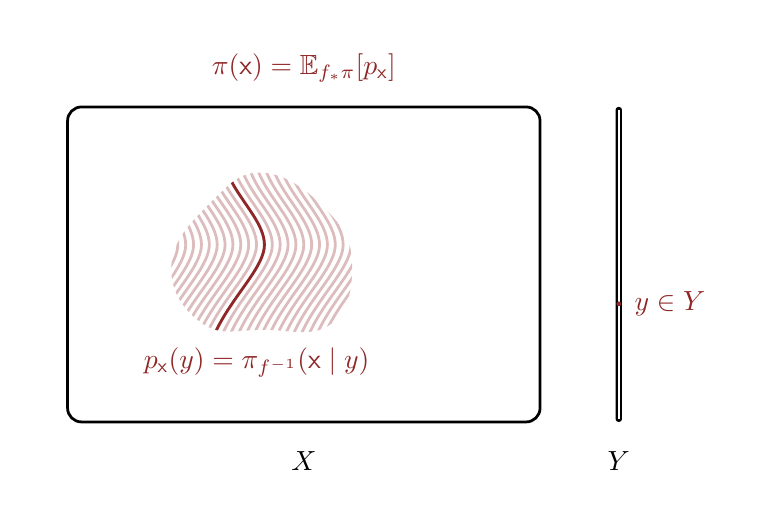
\begin{tikzpicture}[scale=1]

  \draw[white] (-3.5, -3) rectangle (5.5, 3);
   
  % Input Space
  \begin{scope}
    \pgfmathsetseed{11}
    \clip plot [smooth cycle, tension=0.75] coordinates { \randpoints{-0.5}{0}{1} } -- cycle;

    \foreach \x in {-3.4, -3.3, ..., 3.5} {
      \fiber{\x}{light};    
    }  
    \fiber{-1}{dark}; 
  \end{scope}
       
  \node[dark] at (-0.6, -1.25) { $p_{\mathsf{x}}(y) = \pi_{f^{-1}} ( \mathsf{x} \mid y )$ };
  
  \node[dark] at (0, 2.5) { $\pi(\mathsf{x}) = \mathbb{E}_{f_{*} \pi} [ p_{\mathsf{x}}]$ };
  
  
  \draw [rounded corners=5, color=black, line width=1] (-3, -2) rectangle (3, 2);
  \node at (0, -2.5) { $X$ };  
  
  % Output Space
  \fill[rounded corners=1, black] (4 - 0.04, -2) rectangle (4 + 0.04, 2);
  \node[black] at (4, -2.5) { $Y$ }; 
  
  \draw[white, line width=0.75] (4, -2 + 0.04) -- (4, 2 - 0.04);  
  
  \fill[dark] (4, -0.5) circle (0.03);
  \node[dark] at (4.65, -0.5) { $y \in Y$ };

\end{tikzpicture}

\end{document}  